\begin{figure}[ht]
\centering
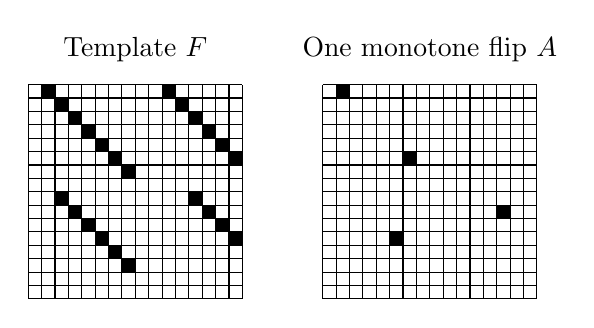
\begin{tikzpicture}[x=0.17cm,y=0.17cm]
\fill (1,15) rectangle ++(1,1);
\fill (10,15) rectangle ++(1,1);
\fill (2,14) rectangle ++(1,1);
\fill (11,14) rectangle ++(1,1);
\fill (3,13) rectangle ++(1,1);
\fill (12,13) rectangle ++(1,1);
\fill (4,12) rectangle ++(1,1);
\fill (13,12) rectangle ++(1,1);
\fill (5,11) rectangle ++(1,1);
\fill (14,11) rectangle ++(1,1);
\fill (6,10) rectangle ++(1,1);
\fill (15,10) rectangle ++(1,1);
\fill (7,9) rectangle ++(1,1);
\fill (2,7) rectangle ++(1,1);
\fill (12,7) rectangle ++(1,1);
\fill (3,6) rectangle ++(1,1);
\fill (13,6) rectangle ++(1,1);
\fill (4,5) rectangle ++(1,1);
\fill (14,5) rectangle ++(1,1);
\fill (5,4) rectangle ++(1,1);
\fill (15,4) rectangle ++(1,1);
\fill (6,3) rectangle ++(1,1);
\fill (7,2) rectangle ++(1,1);
\draw[step=1,thin] (0,0) grid (16,16);
\node[above] at (8,17) {Template $F$};
\fill (23,15) rectangle ++(1,1);
\fill (28,10) rectangle ++(1,1);
\fill (35,6) rectangle ++(1,1);
\fill (27,4) rectangle ++(1,1);
\draw[step=1,thin] (22,0) grid (38,16);
\node[above] at (30,17) {One monotone flip $A$};
\end{tikzpicture}
\caption{The $N=2$ template and the seeded flip used in the CPU tests. Black cells are negative, white cells positive. Rows index lines; columns index points. Only black cells may change. Larger $N$, not this small example, yields the asymptotic counting separation.}
\end{figure}